%%
%% Automatically generated file from DocOnce source
%% (https://github.com/hplgit/doconce/)
%%

% #define PREAMBLE

% #ifdef PREAMBLE
%-------------------- begin preamble ----------------------

\documentclass[%
oneside,                 % oneside: electronic viewing, twoside: printing
final,                   % draft: marks overfull hboxes, figures with paths
10pt,french]{article}

\listfiles               %  print all files needed to compile this document

\usepackage{relsize,makeidx,color,setspace,amsmath,amsfonts,amssymb}
\usepackage[table]{xcolor}
\usepackage{bm,ltablex,microtype}

\usepackage[pdftex]{graphicx}

% Packages for typesetting blocks of computer code
\usepackage{fancyvrb,framed,moreverb}

% Define colors
\definecolor{orange}{cmyk}{0,0.4,0.8,0.2}
\definecolor{tucorange}{rgb}{1.0,0.64,0}
\definecolor{darkorange}{rgb}{.71,0.21,0.01}
\definecolor{darkgreen}{rgb}{.12,.54,.11}
\definecolor{myteal}{rgb}{.26, .44, .56}
\definecolor{gray}{gray}{0.45}
\definecolor{mediumgray}{gray}{.8}
\definecolor{lightgray}{gray}{.95}
\definecolor{brown}{rgb}{0.54,0.27,0.07}
\definecolor{purple}{rgb}{0.5,0.0,0.5}
\definecolor{darkgray}{gray}{0.25}
\definecolor{darkblue}{rgb}{0,0.08,0.45}
\definecolor{darkblue2}{rgb}{0,0,0.8}
\definecolor{lightred}{rgb}{1.0,0.39,0.28}
\definecolor{lightgreen}{rgb}{0.48,0.99,0.0}
\definecolor{lightblue}{rgb}{0.53,0.81,0.92}
\definecolor{lightblue2}{rgb}{0.3,0.3,1.0}
\definecolor{lightpurple}{rgb}{0.87,0.63,0.87}
\definecolor{lightcyan}{rgb}{0.5,1.0,0.83}

\colorlet{comment_green}{green!50!black}
\colorlet{string_red}{red!60!black}
\colorlet{keyword_pink}{magenta!70!black}
\colorlet{indendifier_green}{green!70!white}

% Backgrounds for code
\definecolor{cbg_gray}{rgb}{.95, .95, .95}
\definecolor{bar_gray}{rgb}{.92, .92, .92}

\definecolor{cbg_yellowgray}{rgb}{.95, .95, .85}
\definecolor{bar_yellowgray}{rgb}{.95, .95, .65}

\colorlet{cbg_yellow2}{yellow!10}
\colorlet{bar_yellow2}{yellow!20}

\definecolor{cbg_yellow1}{rgb}{.98, .98, 0.8}
\definecolor{bar_yellow1}{rgb}{.98, .98, 0.4}

\definecolor{cbg_red1}{rgb}{1, 0.85, 0.85}
\definecolor{bar_red1}{rgb}{1, 0.75, 0.85}

\definecolor{cbg_blue1}{rgb}{0.87843, 0.95686, 1.0}
\definecolor{bar_blue1}{rgb}{0.7,     0.95686, 1}

%\setlength{\fboxsep}{-1.5mm}  % adjust cod_vpad/pro_vpad background box

%% Background for code blocks (parameter is color name)

%% pro/cod_vpad: gives some vertical padding before and after the text
%% (but has more simplistic code than _cod/pro_tight+cod/pro).
%% pro/cod_vpad can be used to enclose Verbatim or lst begin/end for code.
%% pro/cod calls _pro/cod_tight and has very little vertical padding,
%% used to enclose Verbatim and other begin/end for code.
%% (pro/cod is what the ptex2tex program could produce with the
%% Blue/BlueBar definitions in .ptex2tex.cfg.)

\newenvironment{cod_vpad}[1]{
   \def\FrameCommand{\colorbox{#1}}
   \MakeFramed{\FrameRestore}}
   {\endMakeFramed}

\newenvironment{_cod_tight}[1]{
   \def\FrameCommand{\colorbox{#1}}
   \FrameRule0.6pt\MakeFramed {\FrameRestore}\vskip3mm}
   {\vskip0mm\endMakeFramed}

\newenvironment{cod}[1]{
\bgroup\rmfamily
\fboxsep=0mm\relax
\begin{_cod_tight}{#1}
\list{}{\parsep=-2mm\parskip=0mm\topsep=0pt\leftmargin=2mm
\rightmargin=2\leftmargin\leftmargin=4pt\relax}
\item\relax}
{\endlist\end{_cod_tight}\egroup}

%% Background for complete program blocks (parameter 1 is color name
%% for background, parameter 2 is color for left bar)
\newenvironment{pro_vpad}[2]{
   \def\FrameCommand{\color{#2}\vrule width 1mm\normalcolor\colorbox{#1}}
   \MakeFramed{\FrameRestore}}
   {\endMakeFramed}

\newenvironment{_pro_tight}[2]{
   \def\FrameCommand{\color{#2}\vrule width 1mm\normalcolor\colorbox{#1}}
   \FrameRule0.6pt\MakeFramed {\advance\hsize-2mm\FrameRestore}\vskip3mm}
   {\vskip0mm\endMakeFramed}

\newenvironment{pro}[2]{
\bgroup\rmfamily
\fboxsep=0mm\relax
\begin{_pro_tight}{#1}{#2}
\list{}{\parsep=-2mm\parskip=0mm\topsep=0pt\leftmargin=2mm
\rightmargin=2\leftmargin\leftmargin=4pt\relax}
\item\relax}
{\endlist\end{_pro_tight}\egroup}

\usepackage{minted}
\usemintedstyle{default}

\usepackage[T1]{fontenc}
%\usepackage[latin1]{inputenc}
\usepackage{ucs}
\usepackage[utf8x]{inputenc}

\usepackage{lmodern}         % Latin Modern fonts derived from Computer Modern

% Hyperlinks in PDF:
\definecolor{linkcolor}{rgb}{0,0,0.4}
\usepackage{hyperref}
\hypersetup{
    breaklinks=true,
    colorlinks=true,
    linkcolor=linkcolor,
    urlcolor=linkcolor,
    citecolor=black,
    filecolor=black,
    %filecolor=blue,
    pdfmenubar=true,
    pdftoolbar=true,
    bookmarksdepth=3   % Uncomment (and tweak) for PDF bookmarks with more levels than the TOC
    }
%\hyperbaseurl{}   % hyperlinks are relative to this root

\setcounter{tocdepth}{2}  % levels in table of contents

% Tricks for having figures close to where they are defined:
% 1. define less restrictive rules for where to put figures
\setcounter{topnumber}{2}
\setcounter{bottomnumber}{2}
\setcounter{totalnumber}{4}
\renewcommand{\topfraction}{0.95}
\renewcommand{\bottomfraction}{0.95}
\renewcommand{\textfraction}{0}
\renewcommand{\floatpagefraction}{0.75}
% floatpagefraction must always be less than topfraction!
% 2. ensure all figures are flushed before next section
\usepackage[section]{placeins}
% 3. enable begin{figure}[H] (often leads to ugly pagebreaks)
%\usepackage{float}\restylefloat{figure}

% --- fancyhdr package for fancy headers ---
\usepackage{fancyhdr}
\fancyhf{} % sets both header and footer to nothing
\renewcommand{\headrulewidth}{0pt}
\fancyfoot[LE,RO]{\thepage}
% Ensure copyright on titlepage (article style) and chapter pages (book style)
\fancypagestyle{plain}{
  \fancyhf{}
  \fancyfoot[C]{{\footnotesize \copyright\ 2019, Ahmed Ammar. Released under CC Attribution 4.0 license}}
%  \renewcommand{\footrulewidth}{0mm}
  \renewcommand{\headrulewidth}{0mm}
}
% Ensure copyright on titlepages with \thispagestyle{empty}
\fancypagestyle{empty}{
  \fancyhf{}
  \fancyfoot[C]{{\footnotesize \copyright\ 2019, Ahmed Ammar. Released under CC Attribution 4.0 license}}
  \renewcommand{\footrulewidth}{0mm}
  \renewcommand{\headrulewidth}{0mm}
}

\pagestyle{fancy}


\usepackage{framed,wrapfig}

% --- begin definitions of admonition environments ---

% Admonition style "grayicon" has colored background, no frame, and an icon
% Admon "notice"
\definecolor{grayicon_notice_background}{rgb}{0.91,0.91,0.91}
% \fboxsep sets the space between the text and the box
\newenvironment{noticeshaded}
{\def\FrameCommand{\fboxsep=3mm\colorbox{grayicon_notice_background}}
 \MakeFramed {\advance\hsize-\width \FrameRestore}}{\endMakeFramed}

\newenvironment{notice_grayiconadmon}[1][À noter]{
\begin{noticeshaded}
\noindent
\begin{wrapfigure}{l}{0.07\textwidth}
\vspace{-13pt}

\includegraphics[width=0.07\textwidth]{latex_figs/small_gray_notice}
\end{wrapfigure} \textbf{#1}\par
\nobreak\noindent\ignorespaces
}
{
\end{noticeshaded}
}

% Admonition style "grayicon" has colored background, no frame, and an icon
% Admon "summary"
\definecolor{grayicon_summary_background}{rgb}{0.91,0.91,0.91}
% \fboxsep sets the space between the text and the box
\newenvironment{summaryshaded}
{\def\FrameCommand{\fboxsep=3mm\colorbox{grayicon_summary_background}}
 \MakeFramed {\advance\hsize-\width \FrameRestore}}{\endMakeFramed}

\newenvironment{summary_grayiconadmon}[1][Résumé]{
\begin{summaryshaded}
\noindent
\begin{wrapfigure}{l}{0.07\textwidth}
\vspace{-13pt}
\includegraphics[width=0.07\textwidth]{latex_figs/small_gray_summary}
\end{wrapfigure} \textbf{#1}\par
\nobreak\noindent\ignorespaces
}
{
\end{summaryshaded}
}

% Admonition style "grayicon" has colored background, no frame, and an icon
% Admon "warning"
\definecolor{grayicon_warning_background}{rgb}{0.91,0.91,0.91}
% \fboxsep sets the space between the text and the box
\newenvironment{warningshaded}
{\def\FrameCommand{\fboxsep=3mm\colorbox{grayicon_warning_background}}
 \MakeFramed {\advance\hsize-\width \FrameRestore}}{\endMakeFramed}

\newenvironment{warning_grayiconadmon}[1][Attention]{
\begin{warningshaded}
\noindent
\begin{wrapfigure}{l}{0.07\textwidth}
\vspace{-13pt}

\includegraphics[width=0.07\textwidth]{latex_figs/small_gray_warning}
\end{wrapfigure} \textbf{#1}\par
\nobreak\noindent\ignorespaces
}
{
\end{warningshaded}
}

% Admonition style "grayicon" has colored background, no frame, and an icon
% Admon "question"
\definecolor{grayicon_question_background}{rgb}{0.91,0.91,0.91}
% \fboxsep sets the space between the text and the box
\newenvironment{questionshaded}
{\def\FrameCommand{\fboxsep=3mm\colorbox{grayicon_question_background}}
 \MakeFramed {\advance\hsize-\width \FrameRestore}}{\endMakeFramed}

\newenvironment{question_grayiconadmon}[1][Question]{
\begin{questionshaded}
\noindent
\begin{wrapfigure}{l}{0.07\textwidth}
\vspace{-13pt}
\includegraphics[width=0.07\textwidth]{latex_figs/small_gray_question2}
\end{wrapfigure} \textbf{#1}\par
\nobreak\noindent\ignorespaces
}
{
\end{questionshaded}
}

% Admonition style "grayicon" has colored background, no frame, and an icon
% Admon "block"
\definecolor{grayicon_block_background}{rgb}{0.91,0.91,0.91}
% \fboxsep sets the space between the text and the box
\newenvironment{blockshaded}
{\def\FrameCommand{\fboxsep=3mm\colorbox{grayicon_block_background}}
 \MakeFramed {\advance\hsize-\width \FrameRestore}}{\endMakeFramed}

\newenvironment{block_grayiconadmon}[1][Block]{
\begin{blockshaded}
\noindent
 \textbf{#1}\par
\nobreak\noindent\ignorespaces
}
{
\end{blockshaded}
}

% --- end of definitions of admonition environments ---

% prevent orhpans and widows
\clubpenalty = 10000
\widowpenalty = 10000

\newenvironment{doconceexercise}{}{}
\newcounter{doconceexercisecounter}


% ------ header in subexercises ------
%\newcommand{\subex}[1]{\paragraph{#1}}
%\newcommand{\subex}[1]{\par\vspace{1.7mm}\noindent{\bf #1}\ \ }
\makeatletter
% 1.5ex is the spacing above the header, 0.5em the spacing after subex title
\newcommand\subex{\@startsection{paragraph}{4}{\z@}%
                  {1.5ex\@plus1ex \@minus.2ex}%
                  {-0.5em}%
                  {\normalfont\normalsize\bfseries}}
\makeatother


% --- end of standard preamble for documents ---


\usepackage[french]{babel}

% insert custom LaTeX commands...

\raggedbottom
\makeindex
\usepackage[totoc]{idxlayout}   % for index in the toc
\usepackage[nottoc]{tocbibind}  % for references/bibliography in the toc

%-------------------- end preamble ----------------------

\begin{document}

% matching end for #ifdef PREAMBLE
% #endif

\newcommand{\exercisesection}[1]{\subsection*{#1}}


% ------------------- main content ----------------------



% ----------------- title -------------------------

\thispagestyle{empty}

\begin{center}
{\LARGE\bf
\begin{spacing}{1.25}
Contrôle continu: Devoir Surveillé N°2
\end{spacing}
}
\end{center}

% ----------------- author(s) -------------------------

\begin{center}
{\bf Ahmed Ammar (\texttt{ahmed.ammar@fst.utm.tn})}
\end{center}

    \begin{center}
% List of all institutions:
\centerline{{\small Institut Préparatoire aux Études Scientifiques et Techniques, Université de Carthage.}}
\end{center}
    
% ----------------- end author(s) -------------------------

% --- begin date ---
\begin{center}
11 Décembre 2019
\end{center}
% --- end date ---

\vspace{1cm}


% FIGURE: [imgs/header2, width=700 frac=1]

% !split


% --- begin exercise ---
\begin{doconceexercise}
\refstepcounter{doconceexercisecounter}

\exercisesection{Exercise \thedoconceexercisecounter: Équation de récurrence (3 points)}


Soit la relation de récurrence suivante:
$$x^{k+2} = 2x^{k+1} - 3x^{k} \ pour \ k \ge 0 \ et \ x^0 =1, \  x^1 =2$$
Calculer et afficher les 10 premiers termes de cette relation sous la forme :
\begin{cod}{cbg_gray}\begin{minted}[fontsize=\fontsize{9pt}{9pt},linenos=false,mathescape,baselinestretch=1.0,fontfamily=tt,xleftmargin=2mm]{text}
x^2 = 1
x^3 = -4
x^4 = -11
x^5 = -10
x^6 = 13
x^7 = 56
x^8 = 73
x^9 = -22
x^10 = -263
x^11 = -460
\end{minted}
\end{cod}
\noindent


% --- begin solution of exercise ---
\paragraph{Solution.}
Le programme qui calcule et affiche les 10 premiers termes de la relation peut s’écrire comme suit:
\begin{pro}{cbg_gray}{bar_gray}\begin{minted}[fontsize=\fontsize{9pt}{9pt},linenos=false,mathescape,baselinestretch=1.0,fontfamily=tt,xleftmargin=2mm]{python}
x0 = 1
x1 = 2
for k in range(10):
 x = 2*x1 - 3*x0
 x0 = x1
 x1 = x
 print("x^{} = {}".format(k+2,x))
\end{minted}
\end{pro}
\noindent

% --- end solution of exercise ---

\end{doconceexercise}
% --- end exercise ---


% !split


% --- begin exercise ---
\begin{doconceexercise}
\refstepcounter{doconceexercisecounter}

\exercisesection{Exercise \thedoconceexercisecounter: Calculer une somme (3 points)}



\subex{a)}
Le code suivant est supposé calculer la somme $s = \sum_{k=1}^M {1\over k}$
\begin{cod}{cbg_gray}\begin{minted}[fontsize=\fontsize{9pt}{9pt},linenos=false,mathescape,baselinestretch=1.0,fontfamily=tt,xleftmargin=2mm]{python}
s = 0;  k = 1;  M = 100
while k < M:
    s += 1/k
print(s)

\end{minted}
\end{cod}
\noindent
Ce programme ne fonctionne pas correctement. Quelles sont les deux erreurs? (si vous essayez d'exécuter le programme, rien ne se passera à l'écran). Écrivez un programme correct.


% --- begin solution of exercise ---
\paragraph{Solution.}
Le programme correct est:
\begin{pro}{cbg_gray}{bar_gray}\begin{minted}[fontsize=\fontsize{9pt}{9pt},linenos=false,mathescape,baselinestretch=1.0,fontfamily=tt,xleftmargin=2mm]{python}
s = 0.;  k = 1;  M = 100
while k <= M:
    s += 1/k
    k+=1
print(s)
\end{minted}
\end{pro}
\noindent

% --- end solution of exercise ---

\subex{b)}
Réécrivez la version corrigée du programme en \textbf{a)} en utilisant une boucle \texttt{for} sur \texttt{k} valeurs au lieu d'une boucle \texttt{while}.


% --- begin solution of exercise ---
\paragraph{Solution.}
La version corrigée du programme dans \textbf{a)} à l'aide d'une boucle \texttt{for} est la suivante:
\begin{pro}{cbg_gray}{bar_gray}\begin{minted}[fontsize=\fontsize{9pt}{9pt},linenos=false,mathescape,baselinestretch=1.0,fontfamily=tt,xleftmargin=2mm]{python}
s = 0.;  M = 100
for k in range(1,M+1):
    s += 1/k
print(s)
\end{minted}
\end{pro}
\noindent

% --- end solution of exercise ---

\end{doconceexercise}
% --- end exercise ---


% !split


% --- begin exercise ---
\begin{doconceexercise}
\refstepcounter{doconceexercisecounter}

\exercisesection{Exercise \thedoconceexercisecounter: Générer des coordonnées équidistantes (4 points)}

\label{ex:coordonnee}

Nous voulons générer $n + 1$ coordonnées $x$ équidistantes dans $[a, b]$. Stocker, pour \texttt{a = -2}; \texttt{b = 3} et \texttt{n= 20} les coordonnées $x$ dans une liste \texttt{xList}.


\subex{a)}
Définir toutes les variables puis utiliser une boucle \textbf{for} et ajouter chaque coordonnée à la liste \texttt{xList} (\emph{initialement vide}).

% --- begin hint in exercise ---

\paragraph{Indication.}
Avec $n$ intervalles, correspondant à $n + 1$ points, dans $[a, b]$, chaque intervalle a une longueur $h = (b-a) / n$. Les coordonnées peuvent alors être générées par la formule \texttt{xi = a + i * h}; $i = 0,…, n$.

% --- end hint in exercise ---


% --- begin solution of exercise ---
\paragraph{Solution.}
La liste \texttt{xList} sera remplis par les valeurs de \texttt{xi} comme suivant:
\begin{cod}{cbg_gray}\begin{minted}[fontsize=\fontsize{9pt}{9pt},linenos=false,mathescape,baselinestretch=1.0,fontfamily=tt,xleftmargin=2mm]{python}
n =20
a, b = -2, 3
h = (b - a) / n
xList = []
for i in range(n+1):
    xi  = a + i * h
    xList.append(xi)
\end{minted}
\end{cod}
\noindent

% --- end solution of exercise ---

\subex{b)}
Utiliser une liste de compréhension comme une implémentation alternative.


% --- begin solution of exercise ---
\paragraph{Solution.}
Nous pouvons également remplir \texttt{xList} par une liste de compréhension:
\begin{cod}{cbg_gray}\begin{minted}[fontsize=\fontsize{9pt}{9pt},linenos=false,mathescape,baselinestretch=1.0,fontfamily=tt,xleftmargin=2mm]{python}
xList = [a + i * h for i in range(n+1)]
\end{minted}
\end{cod}
\noindent

% --- end solution of exercise ---

\subex{c)}
Vectoriser la liste résultante \texttt{xList} en un tableau \texttt{numpy} xVect. N'oubliez pas \textbf{d'importer} d'abord la fonction qui transforme les listes en tableaux à partir de \texttt{numpy}.


% --- begin solution of exercise ---
\paragraph{Solution.}
La fonction \texttt{numpy.array()} transforme les listes en tableaux \texttt{numpy}:
\begin{cod}{cbg_gray}\begin{minted}[fontsize=\fontsize{9pt}{9pt},linenos=false,mathescape,baselinestretch=1.0,fontfamily=tt,xleftmargin=2mm]{python}
from numpy import array
xVect = array(xList)
\end{minted}
\end{cod}
\noindent

% --- end solution of exercise ---

\end{doconceexercise}
% --- end exercise ---


% !split


% --- begin exercise ---
\begin{doconceexercise}
\refstepcounter{doconceexercisecounter}

\exercisesection{Exercise \thedoconceexercisecounter: Implémenter une fonction gaussienne (5 points)}



\subex{a)}
Créer la fonction: \texttt{gauss(x, m = 0, s = 1)}, qui modélise la gaussienne:
\begin{equation}
f(x) =
{1\over\sqrt{2\pi }\, s}
\exp{\left[-\frac{1}{2}\left({x-m\over s}\right)^2\right]}
\end{equation}


% --- begin solution of exercise ---
\paragraph{Solution.}
La fonction \texttt{gauss(x, m = 0, s = 1)} est la suivante:
\begin{cod}{cbg_gray}\begin{minted}[fontsize=\fontsize{9pt}{9pt},linenos=false,mathescape,baselinestretch=1.0,fontfamily=tt,xleftmargin=2mm]{python}
from pylab import *
def gauss(x, m = 0, s = 1):
    A = 1/sqrt(2*pi*s)
    B = -0.5 *((x-m)/s)**2
    return A*exp(B)
\end{minted}
\end{cod}
\noindent

% --- end solution of exercise ---

\subex{b)}
Créer un tableau \texttt{x} à l'aide de la fonction \texttt{linspace}, du module \texttt{numpy}, pour \texttt{100} valeurs \texttt{x} uniformément espacées dans [-10, 10].


% --- begin solution of exercise ---
\paragraph{Solution.}
Pour avoir \texttt{100} valeurs \texttt{x} uniformément espacés dans [-10, 10], on écrit:
\begin{cod}{cbg_gray}\begin{minted}[fontsize=\fontsize{9pt}{9pt},linenos=false,mathescape,baselinestretch=1.0,fontfamily=tt,xleftmargin=2mm]{python}
x = linspace(-10, 10, 100)
\end{minted}
\end{cod}
\noindent

% --- end solution of exercise ---

\subex{c)}
Écrire les instructions pour tracer le graphique ci-dessous à l’aide de la bibliothèque \texttt{matplotlib}.


\vspace{6mm}

% inline figure
\centerline{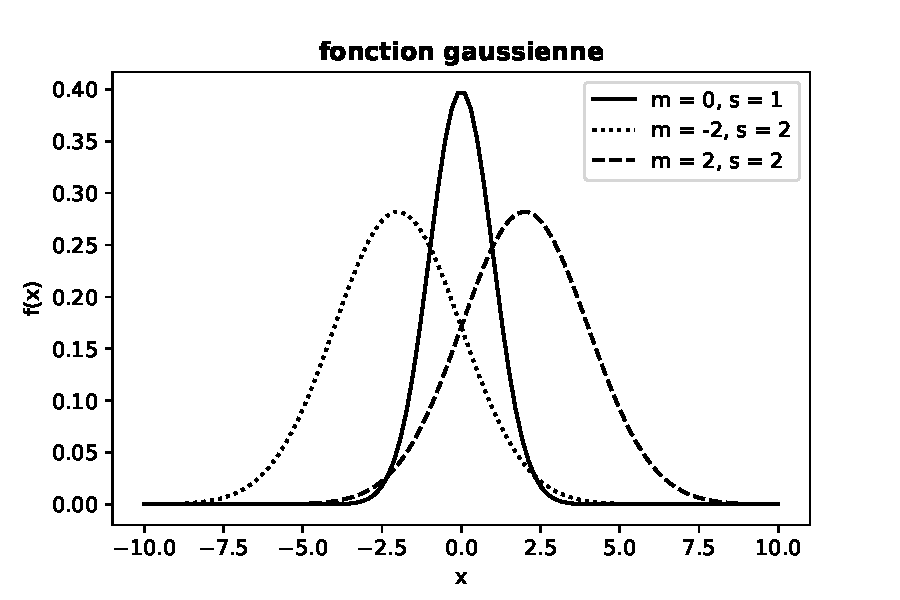
\includegraphics[width=0.7\linewidth]{imgs/gaussian.pdf}}

\vspace{6mm}




% --- begin solution of exercise ---
\paragraph{Solution.}
Le programme qui donne le graphique de la fonction gaussienne est:
\begin{cod}{cbg_gray}\begin{minted}[fontsize=\fontsize{9pt}{9pt},linenos=false,mathescape,baselinestretch=1.0,fontfamily=tt,xleftmargin=2mm]{python}
plt.plot(x, gauss(x, m = 0, s = 1), 'k-', label = 'm = 0, s = 1')
plt.plot(x, gauss(x, m = -2, s = 2), 'k:', label = 'm = -2, s = 2')
plt.plot(x, gauss(x, m = 2, s = 2), 'k--', label = 'm = 2, s = 2')
plt.title("fonction gaussienne", fontweight = 'bold')
plt.xlabel("x")
plt.ylabel("f(x)")
plt.legend()
plt.show()
\end{minted}
\end{cod}
\noindent

% --- end solution of exercise ---

\end{doconceexercise}
% --- end exercise ---


% !split


% --- begin exercise ---
\begin{doconceexercise}
\refstepcounter{doconceexercisecounter}

\exercisesection{Exercise \thedoconceexercisecounter: Tracer les 6 premiers polynômes de Legendre (5 points)}


En mathématiques et en physique théorique, les polynômes de Legendre constituent l'exemple le plus simple d'une suite de polynômes orthogonaux. Ce sont des solutions polynomiales $P_n(x)$ de l'équation différentielle de Legendre :
\begin{equation*}
\frac{d}{d x}\left[(1-x^{2}){\frac {d }{d x}}P_{n}(x) \right]+ n(n+1) P_{n}(x)=0
\end{equation*}
Les polynômes de Legendre sont définis uniquement pour $x \in [-1 ; 1]$ puisque les points $x = \pm 1$ sont des points singuliers réguliers de cette équation différentielle.

Les 6 premiers polynômes de Legendre sont :
\begin{eqnarray*}
P_{0}(x)&=&1 \\\
P_{1}(x)&=&x \\\
P_{2}(x)&=&\frac{1}{2}(3x^{2}-1)\\\
P_{3}(x)&=&\frac{1}{2}(5x^{3}-3x)\\\
P_{4}(x)&=&\frac{1}{8}(35x^{4}-30x^{2}+3)\\\
P_{5}(x)&=&\frac{1}{8}(63x^{5}-70x^{3}+15x)
\end{eqnarray*}


\subex{a)}
Définir les fonctions \texttt{P0(x)}, \texttt{P1(x)}, \texttt{P2(x)}, \texttt{P3(x)}, \texttt{P4(x)} et \texttt{P5(x)} qui retournent les valeurs des 6 premiers polynômes de Legendre.


% --- begin solution of exercise ---
\paragraph{Solution.}
Les fonctions qui calculent les 6 premiers polynômes de Legendre sont les suivantes:
\begin{cod}{cbg_gray}\begin{minted}[fontsize=\fontsize{9pt}{9pt},linenos=false,mathescape,baselinestretch=1.0,fontfamily=tt,xleftmargin=2mm]{python}
import numpy as np
import matplotlib.pyplot as plt
def P0(x):
    return np.ones(len(x))
def P1(x):
    return x
def P2(x):
    return 1/2*(3*x**2 - 1)
def P3(x):
    return 1/2*(5*x**3 - 3*x)
def P4(x):
    return 1/8*(35*x**4 - 30*x**2 + 3)
def P5(x):
    return 1/8*(63*x**5 - 70*x**3 + 15*x)
\end{minted}
\end{cod}
\noindent

% --- end solution of exercise ---

\subex{b)}
Créer un tableau \texttt{x} à l'aide de la fonction \texttt{linspace}, du module \texttt{numpy}, pour \texttt{100} valeurs \texttt{x} uniformément espacées dans [-1, 1].


% --- begin solution of exercise ---
\paragraph{Solution.}
La variable x est définie comme suivant:
\begin{cod}{cbg_gray}\begin{minted}[fontsize=\fontsize{9pt}{9pt},linenos=false,mathescape,baselinestretch=1.0,fontfamily=tt,xleftmargin=2mm]{python}
x=np.linspace(-1,1,100)
\end{minted}
\end{cod}
\noindent

% --- end solution of exercise ---

\subex{c)}
Tracer ces polynômes sur le même graphique en utilisant la bibliothèque \texttt{matplotlib}.


% --- begin solution of exercise ---
\paragraph{Solution.}
Les instructions pour le traçage des courbes sont les suivantes:
\begin{cod}{cbg_gray}\begin{minted}[fontsize=\fontsize{9pt}{9pt},linenos=false,mathescape,baselinestretch=1.0,fontfamily=tt,xleftmargin=2mm]{text}
plt.figure()
plt.plot(x,P0(x),label='P0')
plt.plot(x,P1(x),label='P1')
plt.plot(x,P2(x),label='P2')
plt.plot(x,P3(x),label='P3')
plt.plot(x,P4(x),label='P4')
plt.plot(x,P5(x),label='P5')
plt.title('Les six premiers polynômes de Legendre', weight = "bold")
plt.xlabel("x")
plt.ylabel("P(x)")
plt.legend()
plt.grid()
plt.show()
\end{minted}
\end{cod}
\noindent


\begin{notice_grayiconadmon}[À noter]
Voici l'ensemble des solutions des questions a), b) et c) dans un script \texttt{PolyLegendre.py}:
\begin{pro}{cbg_gray}{bar_gray}\begin{minted}[fontsize=\fontsize{9pt}{9pt},linenos=false,mathescape,baselinestretch=1.0,fontfamily=tt,xleftmargin=2mm]{python}
## NOM DU PROGRAMME: PolyLegendre.py
#% IMPORTATION
import numpy as np
import matplotlib.pyplot as plt
def P0(x):
    return np.ones(len(x))
def P1(x):
    return x
def P2(x):
    return 1/2*(3*x**2 - 1)
def P3(x):
    return 1/2*(5*x**3 - 3*x)
def P4(x):
    return 1/8*(35*x**4 - 30*x**2 + 3)
def P5(x):
    return 1/8*(63*x**5 - 70*x**3 + 15*x)
x=np.linspace(-1,1,100)
plt.figure()
plt.plot(x,P0(x),label='P0')
plt.plot(x,P1(x),label='P1')
plt.plot(x,P2(x),label='P2')
plt.plot(x,P3(x),label='P3')
plt.plot(x,P4(x),label='P4')
plt.plot(x,P5(x),label='P5')
plt.title(u'Les six premiers polynômes de Legendre', weight = "bold")
plt.xlabel("x")
plt.ylabel("P(x)")
plt.legend()
plt.grid()
plt.savefig("legendre.png"); plt.savefig("legendre.pdf")
plt.show()
\end{minted}
\end{pro}
\noindent
\end{notice_grayiconadmon} % title: À noter



% --- end solution of exercise ---

\end{doconceexercise}
% --- end exercise ---


% ------------------- end of main content ---------------

% #ifdef PREAMBLE
\end{document}
% #endif

